\begin{frame}\begin{center}
		\LARGE\textbf{Life-cycle of earnings}
\end{center}\end{frame}
%-------------------------------------------------------------------------------
%-------------------------------------------------------------------------------
\begin{frame}\textbf{Stylized Facts}\vspace{0.3cm}

\begin{itemize}\setlength\itemsep{1em}
\item Life-cycle earnings are increasing at early ages and decline towards the end.
\item Wages tend to increase over the life-cycle with a weak tendency to decline at the end of working life.
\item Hours of work increase at early ages and decline in old age, with the peak occurring earlier than in the wage profiles.
\end{itemize}

See \citeA{Weiss.1986} for comprehensive modeling framework that allows to interpret all these facts.
\end{frame}
%-------------------------------------------------------------------------------
%-------------------------------------------------------------------------------
\begin{frame}
	\begin{figure}[htp]\centering
		\caption{Wage gains}\scalebox{0.35}
		{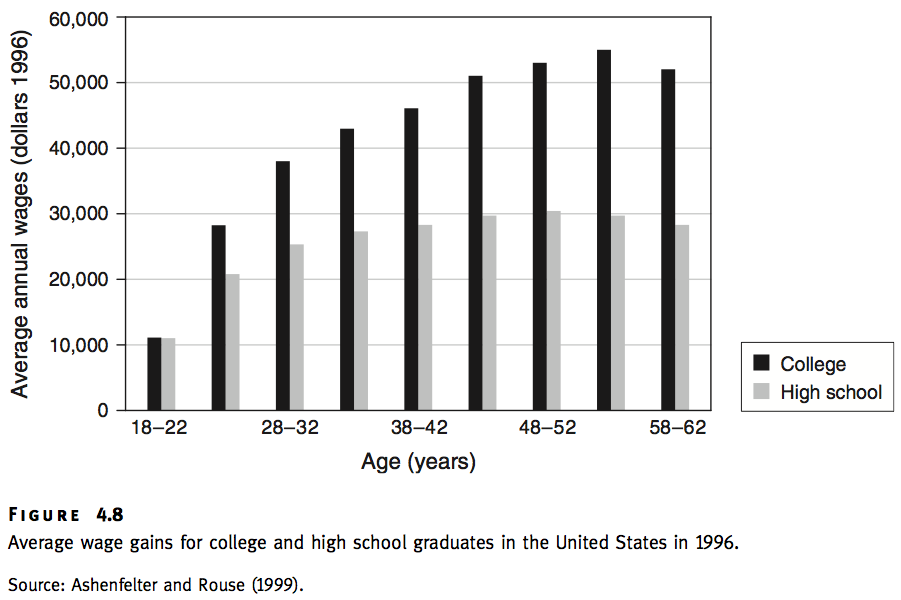
\includegraphics{fig-wage-gains}}
	\end{figure}
\end{frame}
%-------------------------------------------------------------------------------
%-------------------------------------------------------------------------------
\begin{frame}
We study a version of the seminal Ben-Porath Model \cite{Ben-Porath.1967} that relates human capital accumulation to life-cycle earnings. \\\vspace{1cm}

Why do economists use mathematical models? (\href{https://github.com/HumanCapitalAnalysis/talks/blob/master/distribution/research_skills/02_mathematical_modeling.pdf}{slides})
\end{frame}
%-------------------------------------------------------------------------------
%-------------------------------------------------------------------------------
\begin{frame} This material is best studied using the following resource.\\\vspace{0.3cm}

\begin{itemize}
\item \bibentry{Cahuc.2004}
\end{itemize}

\end{frame}
%-------------------------------------------------------------------------------
%-------------------------------------------------------------------------------
\begin{frame}\textbf{Basic Notation}\vspace{0.3cm}
\begin{align*}\begin{array}{l@{\qquad}l@{\qquad}l}
s(t) 	& \text{fraction devoted to training} \\
h(t)    & \text{stock of human capital} \\
w(t)	& \text{wage} \\
\delta  & \text{depreciation of knowledge}
\end{array}\end{align*}
\end{frame}
%-------------------------------------------------------------------------------
%-------------------------------------------------------------------------------
\begin{frame}
The individual's objective is to maximize the discounted sum of wages over their life-cycle.

\begin{align*}
\Omega = \int^T_0 w(t)\, e^{-r t} dt
\end{align*}
\end{frame}

\begin{frame}
Their economic environment is characterized by the production functions for wages and human capital.

\begin{align*}
w(t)    & = A[1 - s(t)]h(t) \\
\dot{h} & = \theta g(s(t),h(t)) - \delta h(t) \qquad g^\prime > 0, g^{\prime\prime} < 0
\end{align*}

\end{frame}
%-------------------------------------------------------------------------------
%-------------------------------------------------------------------------------
\begin{frame}\textbf{Notable Features}\vspace{0.3cm}

\begin{itemize}\setlength\itemsep{1em}
\item Individuals cannot work and learn at the same time.
\item There is no individual heterogeneity.
\item There is no direct cost of education but there are the opportunity cost of lost wages.
\item $\hdots$
\end{itemize}

\end{frame}
%-------------------------------------------------------------------------------
%-------------------------------------------------------------------------------
\begin{frame}\textbf{Model Specification}\vspace{0.3cm}

We study the implementation in \citeA{Cahuc.2004}.

\begin{align*}
	g(h(t), s(t) = \left(h(t) s(t)\right)^{0.71}
\end{align*}\vspace{-1.0cm}
\begin{align*}\begin{array}{l@{\qquad}l@{\qquad}l}
	A = 0.75 & \delta = 0.06 & r = 0.05\\
	h_0 = 5 & T = 60 & \theta = 0.5
\end{array}\end{align*}
\end{frame}

\begin{frame}\begin{figure}[htp]\centering
\caption{Contour plot of human capital production function}
\scalebox{0.35}{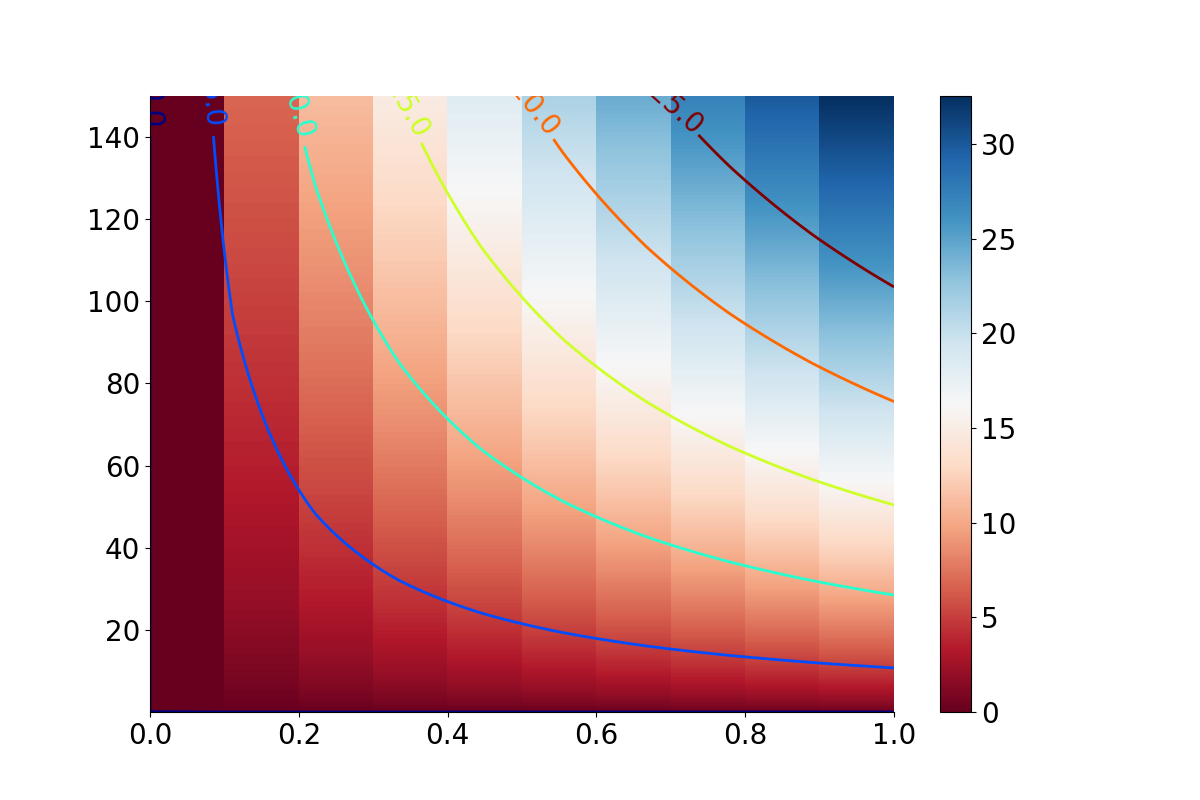
\includegraphics{fig-model-porath-production-intensity}}
\end{figure}\end{frame}

\begin{frame}\begin{figure}[htp]\centering
\caption{Surface plot of human capital production function}
\scalebox{0.35}{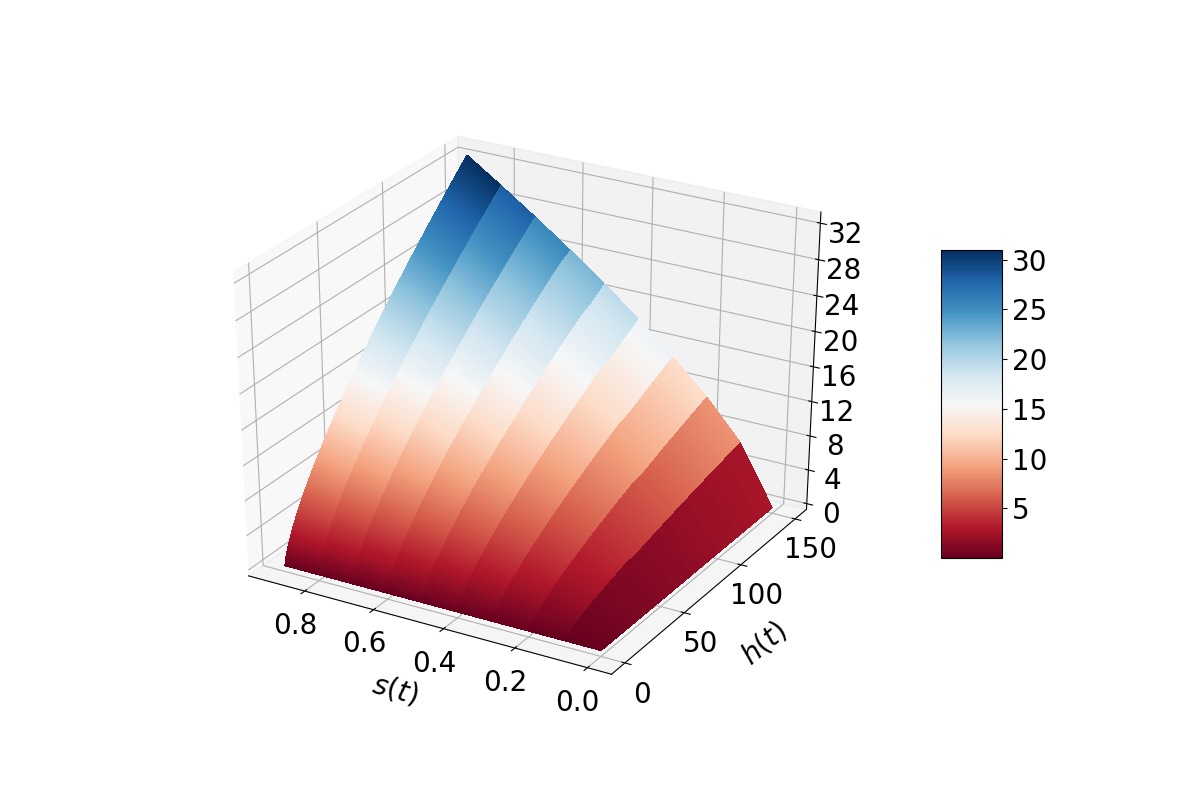
\includegraphics{fig-model-porath-production-surface}}
\end{figure}\end{frame}

\begin{frame}\begin{figure}[htp]\centering
\caption{Wage production}
\scalebox{0.35}{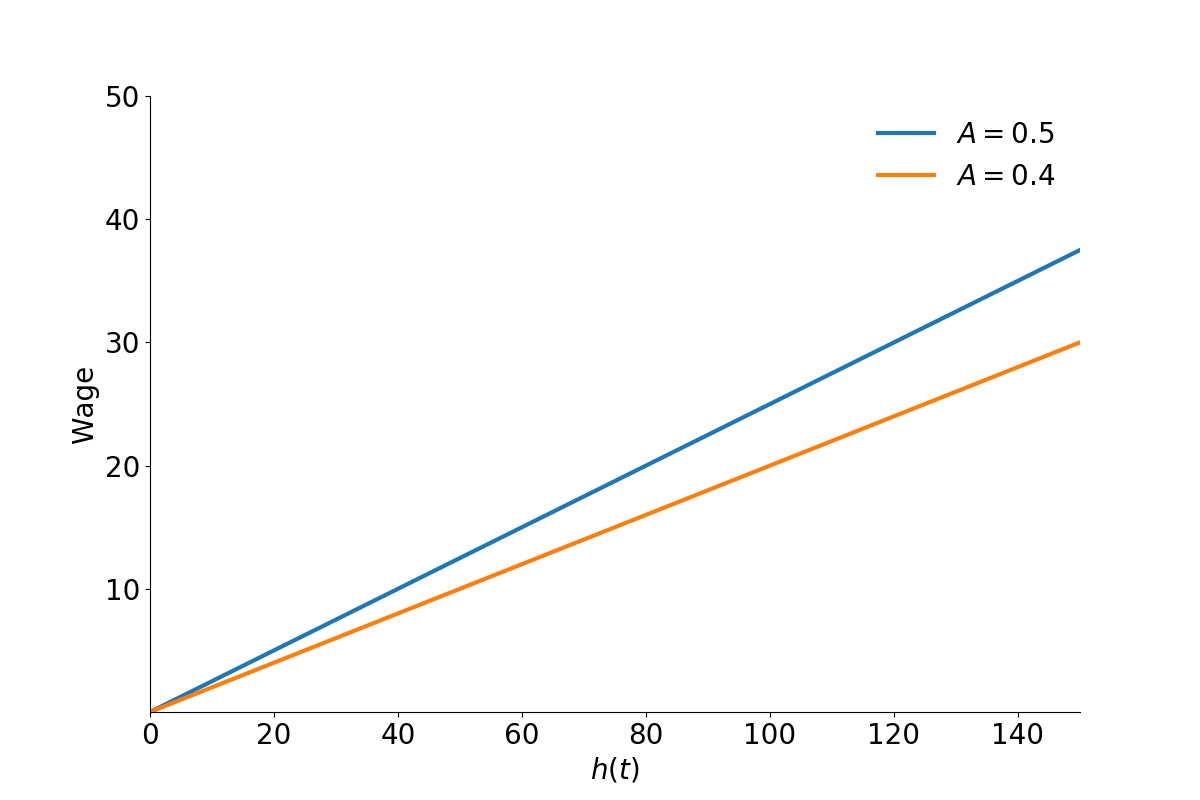
\includegraphics{fig-model-porath-wage}}
\end{figure}\end{frame}

\begin{frame}\begin{figure}[htp]\centering
\caption{Wage $w(t)$ over the life-cycle}
\scalebox{0.35}{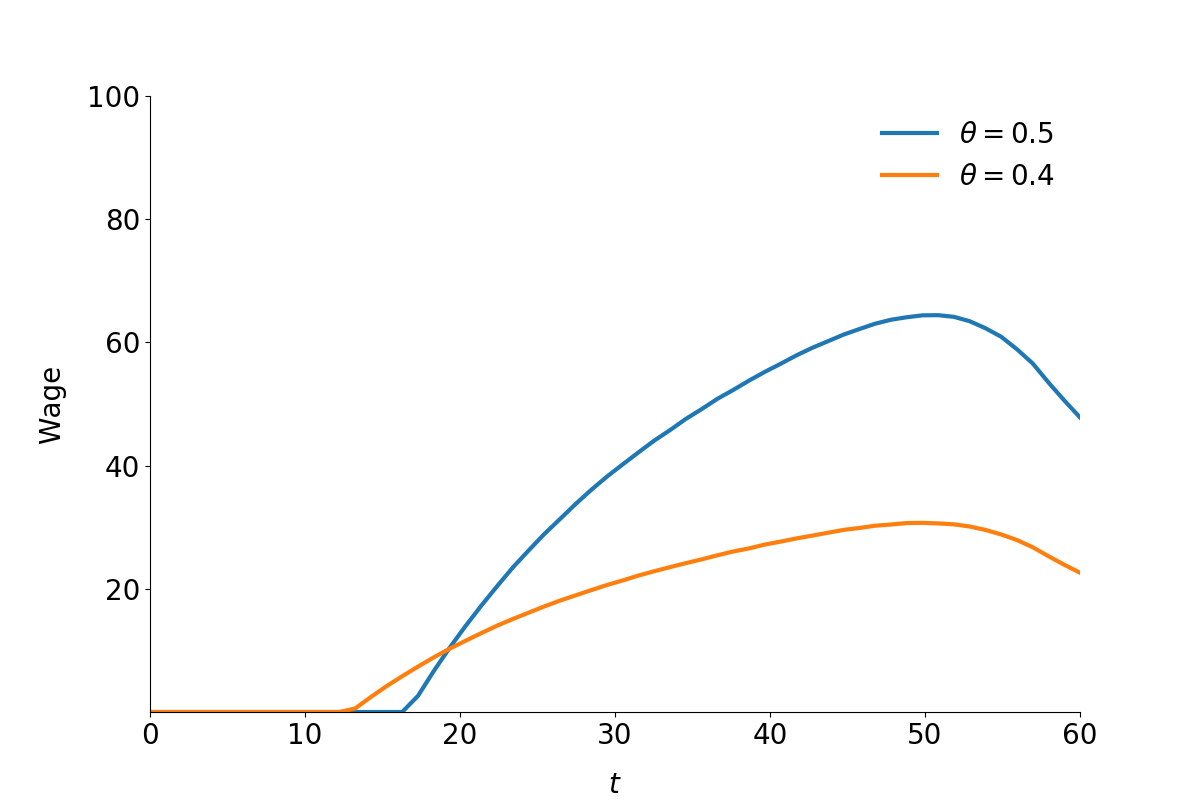
\includegraphics{fig-model-porath-life-cycle-wage}}
\end{figure}\end{frame}

\begin{frame}\begin{figure}[htp]\centering
\caption{Stock of human capital $h(t)$ over the life-cycle}
\scalebox{0.35}{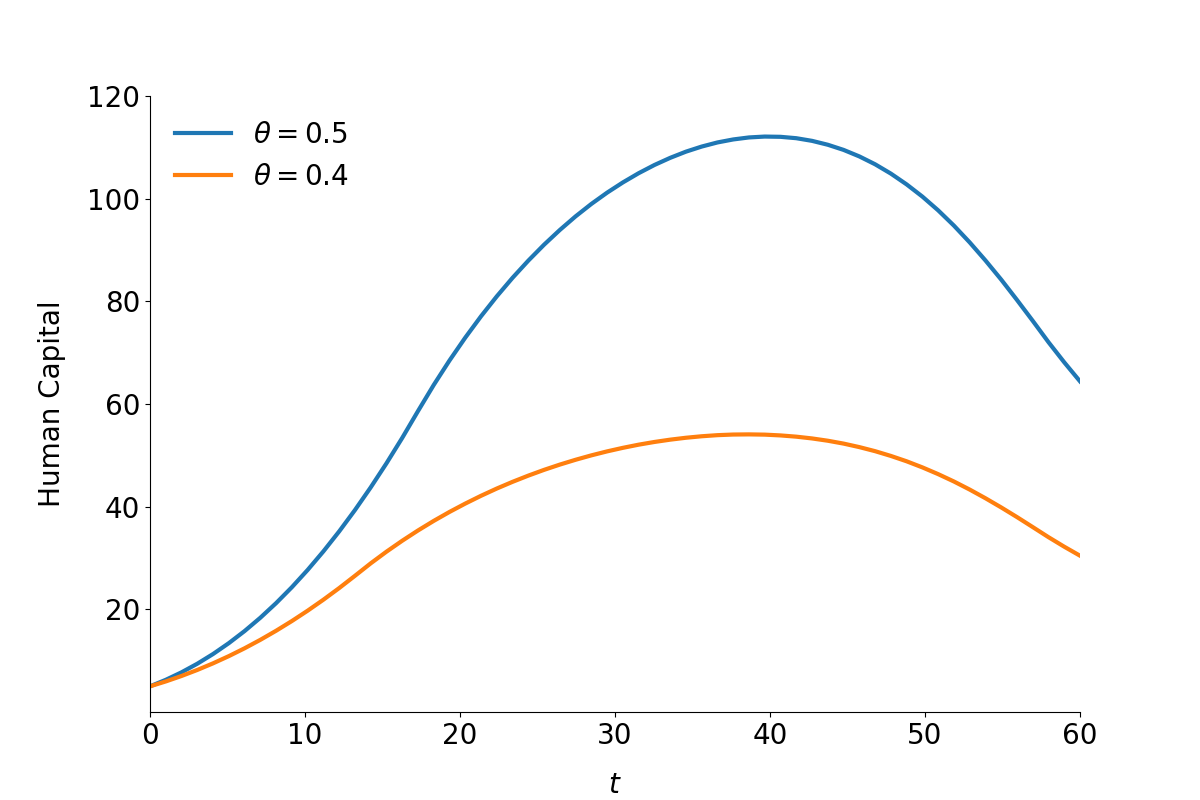
\includegraphics{fig-model-porath-life-cycle-stock}}
\end{figure}\end{frame}

\begin{frame}\begin{figure}[htp]\centering
\caption{Human capital investment $s(t)$ over the life-cycle}
\scalebox{0.35}{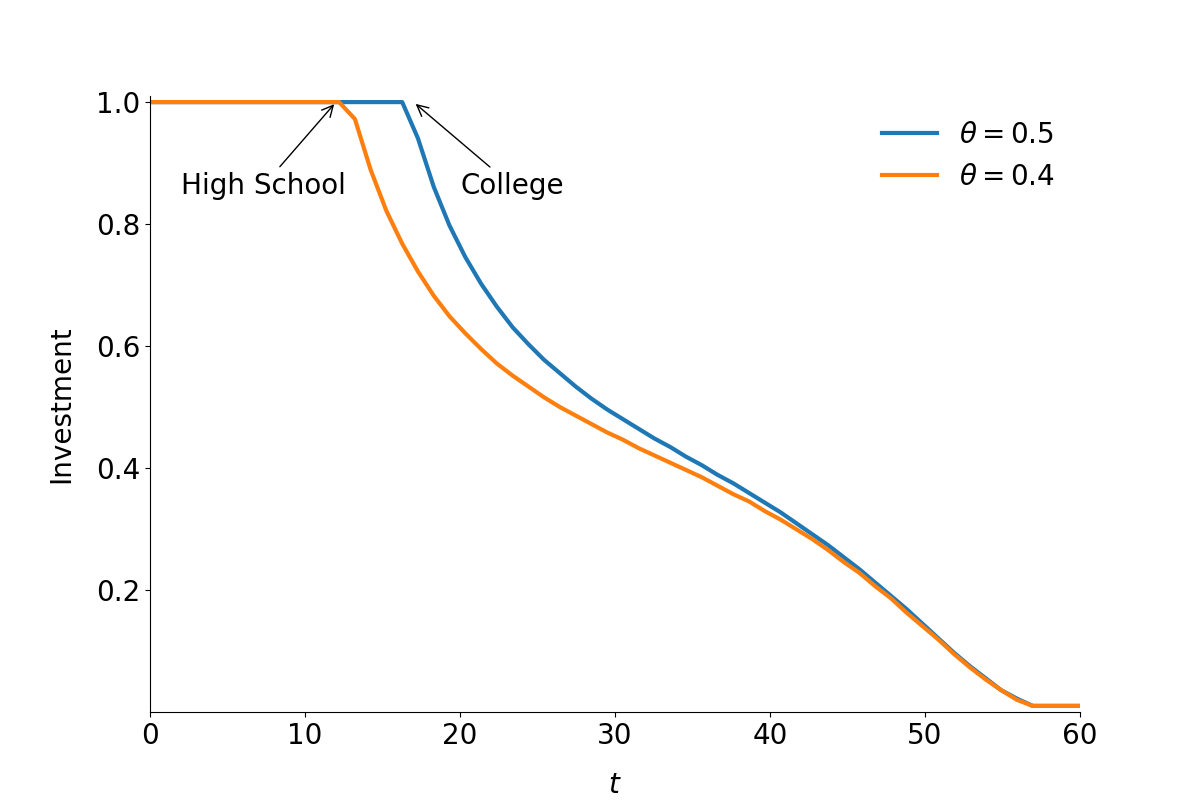
\includegraphics{fig-model-porath-life-cycle-investment}}
\end{figure}\end{frame}

\begin{frame}\begin{figure}[htp]\centering
\caption{Hours worked $(1 - s(t))$ over the life-cycle}
\scalebox{0.35}{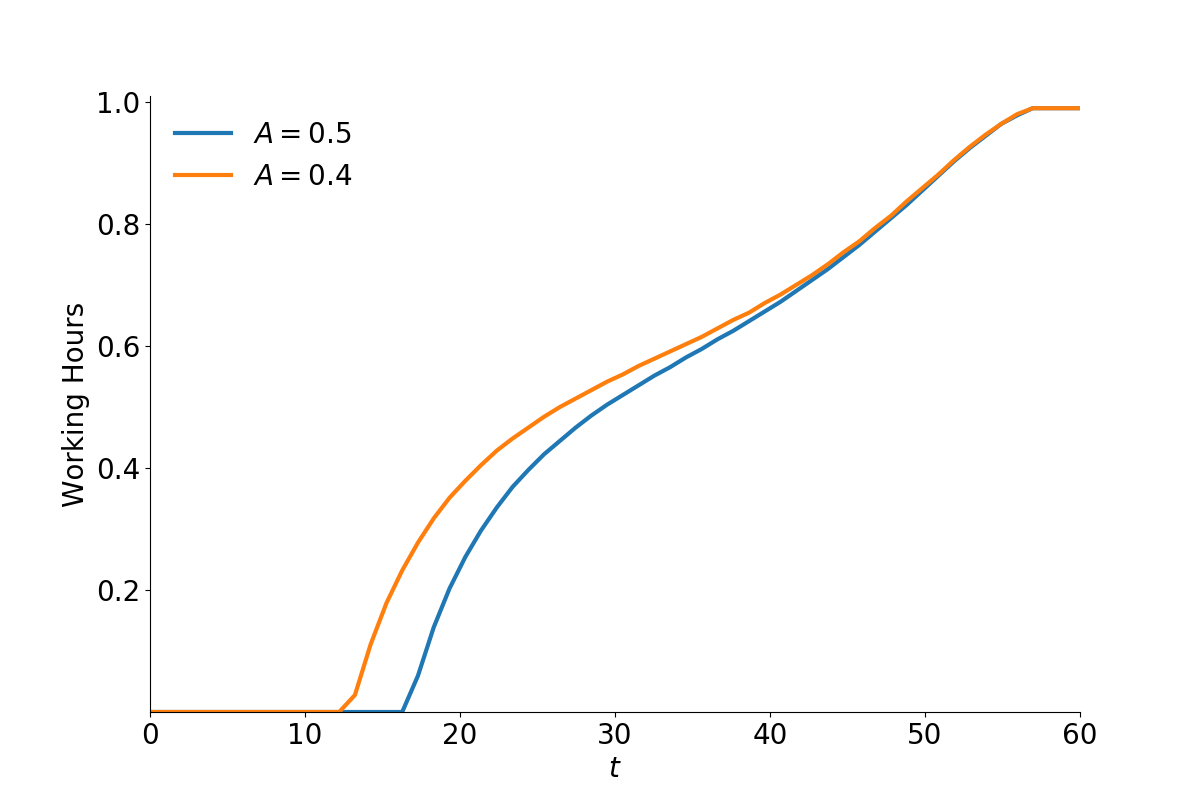
\includegraphics{fig-model-porath-life-cycle-hours}}
\end{figure}\end{frame}

\begin{frame}\begin{figure}[htp]\centering

How well does the model do?

\end{figure}\end{frame}
%-------------------------------------------------------------------------------
%-------------------------------------------------------------------------------
\begin{frame}\textbf{Extensions}\vspace{0.3cm}

\citeA{Weiss.1986} reviews a host of alternative extensions to the basic model.\\

\begin{itemize}\setlength\itemsep{1em}
\item general versus specific training
\item hours worked
\item uncertainty
\item borrowing-constraints
\item $\hdots$
\end{itemize}

\end{frame}
